\documentclass{ctexart}
\usepackage{graphicx}
\usepackage[colorlinks,linkcolor=black,anchorcolor=black,citecolor=black]{hyperref}
\usepackage{amsmath}

\begin{document}
\title{卡尔曼滤波(kalman filter)}
\author{ }
\maketitle

\newpage
\section{简介}
卡尔曼滤波是一种滤波算法或数据融合算法.通常是将多组数据融合以求获得最接近真实值的结果.

卡尔曼有五个公式,可以划分为\emph{预测}和\emph{修正}两部分.

其中预测部分,是靠物体内部数据(或着说第一组数据)对其下一步运动状态进行估计,但是这个估计往往是不准确的,并且假设其误差服从正态分布.

而修正部分,是靠物体外部数据(或第二组数据)对预测部分进行修正.但是,外部数据往往也是不准确的,并且也需要假设其误差服从正态分布.\emph{重要的是,第一组数据和第二组数据的误差\footnote{和客观真实值之间的误差}是相互独立的,如此一来,结合两组数据便可以缩小误差.}

\section{原理和推导}
假设物体某一刻的状态的估计值为$\hat x$,通常为是多维向量.比如$\hat x$可以是某时刻$t$物体的运动速度$v$和加速度$a$组成.
$$\hat x=
 \left[
 \begin{array}{c}
   v \\
   a	
 \end{array}
 \right]
$$
根据物体的运动状态,可以对物体下一时刻$t+1$的状态进行预测
$$
 \left[\begin{array}{c}
   v_{t+1} \\
   a_{t+1}	
 \end{array}\right]
 =
 \left[\begin{matrix}
 	1 & \Delta t \\
 	0 & 1
 \end{matrix}\right]
 \left[\begin{array}{c}
   v_{t} \\
   a_{t}
 \end{array}\right]
$$即
$$\hat x_{t+1}=A\hat x_{t}$$
需要的话,上式需要加上控制量$u_t$,表示外界变量\footnote{如人为控制物体加速减速等}对物体运动状态的影响.
\begin{equation}
\hat x_{t+1}=A\hat x_{t}+Bu_{t}	
\end{equation}

现实情况下,估计值$\hat x_{t+1}$和真实值$x_{t+1}$之间存在一个误差,误差用$w_t$表示,且该误差服从高斯分布.
% TODO 写这里
这里还需要对估计值$\hat x_{t+1}$的协方差矩阵进行分析.

如图\ref{xt-xt+1}所示,物体从$x_t$运动到$x_{t+1}$,由于误差的存在,$x_{t+1}$并非是确定的,而往往是一定范围中的某点,该范围用图中虚线椭圆表示.
\begin{figure}[hbt]
  \centering
  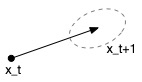
\includegraphics{img/xt+1.jpg}
  \caption{物体运动}
  \label{xt-xt+1}
\end{figure}

此时还需要关注一下$w_t$,$w_t$是多维向量的误差,所以$w_t\sim N(0,Q_t)$,它有一个协方差矩阵\footnote{参阅概率论.一维变量有\emph{期望}和\emph{方差},多维随机变量有\emph{期望向量}和\emph{协方差矩阵}}$Q_t$,在本例中
$$Q_t=
 \left[\begin{matrix}
 	\sigma_{11} & \sigma_{12} \\
 	\sigma_{21} & \sigma_{22}
 \end{matrix}\right]
$$
其中$\sigma_{11}$和$\sigma_{22}$分别是$v$和$a$的方差,而$\sigma_{12}=\sigma_{21}$是$v$和$a$协方差,数值相等.

设$x_t$的协方差矩阵为$P_t$



\bibliographystyle{plain}
\bibliography{refs.bib}
	
\end{document}